
\section{Robustness of modeling results}
\label{metabolism:robust}

We conducted numerous parameter sweeps to confirm the robustness of each result presented in this chapter. In each sweep, all model parameters were varied across a ten-fold range ($\pm \sim$three-fold). To efficiently sample the parameter space, we quasi-randomly sampled 2500 parameter sets from the multi-dimensional hyperspace defined by one order of magnitude variation in each of the model parameters. For each parameter set we independently ran six sets of five thousand simulations: 
\begin{enumerate}
	\item Full feedback with normal metabolism and translation
	\item Partial feedback with normal metabolism and translation
	\item Full feedback with reduced energy metabolism
	\item Partial feedback with reduced energy metabolism
	\item Full feedback with reduced protein synthesis	
	\item Partial feedback with reduced protein synthesis
\end{enumerate}

Full-repression systems were assigned two copies of each feedback element present in the corresponding partial-repression system. Error frequencies were evaluated as described previously. In total, this procedure constitutes one parameter sweep. 

Our parameter sweeps sampled an $N$-dimensional space, prompting us to seek a lower dimensional representation in order to visualize and discern any characteristic trends. One option is to project the results of each simulation onto the $N(N-1)/2$ unique two-dimensional planes. Figure \ref{fig:metabolism:figS1b}A provides an example of this visualization applied to error frequencies simulated with partial feedback and normal metabolism. While it is clear that error frequency is greater than 1\% for most combinations of parameter values, we find that the complexity of the 2-D visualization offers little additional insight. Instead, for all remaining parameter sweeps we opt for the simpler one dimensional projection of parameter sweep results, as illustrated by Figure \ref{fig:metabolism:figS1b}B. The histogram simply conveys the global trend in simulated error frequency, which in this case is skewed heavily toward large error frequencies, indicating that partial loss of repression induces an increase in error frequency across a broad parameter range. 

\begin{figure}[h!]
\centering
\includegraphics[scale=1.0]{./figure_S1b}
\caption[Robustness of reduced metabolism simulations to parameter values.]{\textbf{Error frequencies are broadly increased when an auxiliary repressor is lost.} (A) Simulated error frequencies are projected onto two dimensional planes and then linearly interpolated onto (100 px)\textsuperscript{2} grids. (B) Binned counts of the 2500 simulated error frequencies depicted in A. The majority of parameter sets yield high error frequencies.}
\label{fig:metabolism:figS1b}
\end{figure}

We also varied the level of the success threshold, and recalculated all error frequencies accordingly. Error frequency is greater than 1\% for almost all definitions of the success threshold, indicating that loss of a repressor increases developmental error irrespective of where the success threshold is set (Fig. \ref{fig:metabolism:figS1c}).

\begin{figure}[h!]
\centering
\includegraphics[scale=1.0]{./figure_S1c}
\captionsetup{width=.65\linewidth}
\caption[Robustness of reduced metabolism simulations to threshold definition.]{\textbf{Error frequencies increase when a repressor is lost irrespective of where the success threshold is set.} Error frequencies for parameter sets from Fig. \ref{fig:metabolism:figS1b} were re-calculated across a range of different success thresholds. Thresholds are defined by the 99\textsuperscript{th} percentile of protein levels simulated with all repressors, and are evaluated at the time when the mean protein level with all repressors reaches the indicated fraction of its maximum value. Each line represents one of the parameter sets from Figure \ref{fig:metabolism:figS1b}. Color scale reflects maximum difference in error frequency across the range of thresholds tested.}
\label{fig:metabolism:figS1c}
\end{figure}

We also surveyed how error frequency changes when metabolism is reduced. For the control theoretic model, error frequencies simulated across the parameter space were heavily skewed toward lower values (Fig. \ref{fig:metabolism:figS2a}A). For each parameter set, we then computed the difference in simulated error frequency between conditions of normal and reduced energy metabolism. The one-dimensional representation clearly shows that simulated error frequency decreases when metabolism is reduced for the vast majority of the sampled parameter space (Fig. \ref{fig:metabolism:figS2a}B). Similarly, simulated error frequency decreases when metabolism is reduced regardless of where the threshold is set (Fig. \ref{fig:metabolism:figS2a}C). 

Our conclusion also persists when a nonzero basal stimulus is introduced. We conducted an additional parameter sweep in which the stimulus consists of a transient step change between input values of $\Delta I=0.1$ and $\Delta I=1.0$. Simulations were carried out on an absolute basis, and were allowed sufficient time to reach a non-zero steady state before and after the stimulus was applied. The resultant protein level trajectories for each of the six sets of simulations were converted to deviation form by subtracting the respective population-wide mean final value. Error frequencies were then evaluated as previously described. Despite the inclusion of a nonzero basal stimulus, error frequencies remained broadly suppressed under conditions of reduced energy metabolism (Fig. \ref{fig:metabolism:figS2a}C).

All preceding simulations assume the stimulus (input) is a unit step that persists for three hours regardless of metabolic conditions. Alternatively, metabolic conditions might affect stimulus (input) duration, particularly if the upstream processes responsible for the input are also governed by metabolically delayed processes. We find that the general prediction made by our model -- that reduced energy metabolism and reduced protein synthesis limit sensitivity to loss of regulation -- persists in roughly half of cases if we apply a four-fold extension of input duration when energy metabolism is reduced (Fig. \ref{fig:metabolism:figS2a}E). Notably, in many cases scaling the input duration with metabolic condition yields the opposite effect. However, these instances correspond to simulations in which the extended stimulus yields output protein levels greater than those observed under normal metabolic conditions, suggesting that a four-fold increase in stimulus duration may be excessive. Nevertheless, we take this to be an upper bound on the observed phenotype suppression phenomenon.

Our control theoretic modeling framework suffers two notable limitations. First, the number of transcriptionally active sites within a cell is limited by gene copy number, but the activated-DNA state in our initial linear model was unbounded. To test whether error frequency suppression persists when an upper bound on gene activity is introduced, we considered a simple two-state transcription model:
\begin{equation}
\begin{aligned}
\label{appendix:supp:metabolism:model:twostate_eqns}
\frac{dG_{on}}{dt} &= k_{G}G_{off}I -\gamma_G G_{on} - \sum^{N_g}{\eta_{G} G_{on}P} \\
\frac{dG_{off}}{dt} &= -\frac{dG_{on}}{dt} \\
\frac{dR}{dt} &= k_{R} G_{on} -\gamma_R R -\sum^{N_r}{\eta_{R} P} \\
\frac{dP}{dt} &= k_{P} R -\gamma_P P -\sum^{N_p}{\eta_{P} P}
\end{aligned}
\end{equation}
where $G_{on}$ and $G_{off}$ are the on- and off- states of a gene; $I$, $R$, and $P$ are the input, transcript, and protein levels; $k_i$, $\gamma_i$, and $\eta_i$ are the synthesis, decay, and feedback rate constants for species $i$; and $N_g$, $N_r$, and $N_p$ are the number of transcriptional, post-transcriptional, and post-translational repressors, respectively. Rate parameter dependencies upon environmental conditions were analogous to those used in the linear model, and are listed in Table \ref{appendix:supp:metabolism:model:metabolism_twostate}. We performed another parameter sweep varying each of the model's nine parameters across one order of magnitude. All simulations were initialized as diploid ($G_{off}=2$) then subject to a constant 3 h stimulus before reverting to a basal level of zero gene expression. Despite the limitation placed on gene activity, error frequency remained elevated under normal growth conditions and broadly suppressed when ATP-dependent rate parameters were reduced (Fig. \ref{fig:metabolism:figS2a}F).

Second, gene expression models frequently utilize cooperative kinetics in order to reproduce the nonlinearities and thresholds encountered in transcriptional regulation. We captured these dynamics by reformulating our model in terms of Hill kinetics:
\begin{equation}
\begin{aligned}
\label{appendix:supp:metabolism:model:hill_eqns}
\frac{dR}{dt}&=\frac{k_{R}}{1+(\frac{1}{2I})^H}\prod^{N_g}{\Bigg[\frac{1}{1+(\frac{P}{K_{r}})^{H_{r}}}\Bigg]} -\gamma_R R - \sum^{N_r}{\eta_{R} P} \\
\frac{dP}{dt}&=k_{P}R -\gamma_P P - \sum^{N_p}{\eta_{P} P}
\end{aligned}
\end{equation}
where $I$, $R$, and $P$ are the input, transcript, and protein levels; $k_i$, $\gamma_i$, and $\eta_i$ are the synthesis, decay, and linear feedback rate constants for species $i$; $N_r$ and $N_p$ are the number of post-transcriptional, and post-translational linear repressors; $H$ is a transcriptional Hill coefficient; and $K_r$ and $H_r$ are the half-maximal occupancy level and Hill coefficient of each of the $N_g$ transcriptional repressors. The stimulus level corresponding to half-maximal transcription rate was fixed at 0.5 because we only consider a binary input signal. Rate parameters were again scaled with metabolic and protein synthesis conditions in a manner analogous to the linear model, as listed in Table \ref{appendix:supp:metabolism:model:metabolism_hill}. Despite the incorporation of cooperative kinetics, error frequencies remained elevated under normal conditions and broadly suppressed when ATP-dependent rate parameters are reduced (Fig. \ref{fig:metabolism:figS2a}G).

\begin{figure}[h!]
\centering
\includegraphics[width=1.0\columnwidth]{./figure_S2a}
\caption[Robustness of reduced metabolism simulations to model assumptions.]{\textbf{Reduced energy metabolism diminishes the importance of auxiliary repressors over a wide range of model conditions.} (A-G) For each panel, 2500 simulations were performed with parameter sets quasi-randomly sampled from the nine-dimensional hyperspace defined by one order of magnitude variation in each of the respective model parameters, as done for Fig. \ref{fig:metabolism:figS1b}. For each parameter set, error frequencies pertain to 50\% loss of repression mimicking partial repressor loss. (A) One-dimensional representation of the error frequencies for all parameter sets under conditions of normal or diminished energy metabolism. (B) Change in error frequencies with diminished metabolism relative to normal metabolic conditions for all parameter sets. Blue-Red color scale corresponds to the difference in error frequency between low-metabolic and normal conditions, e.g. blue indicates error suppression by reduced energy metabolism. (C) Results from (B) re-calculated across a range of different success thresholds. Each line corresponds to a single parameter set. Color scale reflects maximum change in error frequency across the threshold range. Black dashed line corresponds to unchanged error frequency by reduced energy metabolism. The vast majority of simulations exhibit some reduction in error frequency across all thresholds. (D-G) Systematic modification of model conditions showing the change in error frequencies with diminished metabolism relative to normal metabolic conditions for all parameter sets. Blue-Red color scale corresponds to the difference in error frequency between low-metabolic and normal conditions, e.g. blue indicates error suppression by reduced energy metabolism. (D) Simulations where a nonzero basal stimulus is applied. (E) Simulations where input duration is increased four-fold by a reduction in energy metabolism. (F) Simulations when an upper bound is placed on the number of sites firing transcription. (G) Simulations when cooperative transcription kinetics are considered.}
\label{fig:metabolism:figS2a}
\end{figure}

Our simulations revealed that protein expression is less sensitive to repressor loss when metabolic conditions are reduced (Fig. \ref{fig:metabolism:figS3a}). We computed the same protein overexpression metric for each set of simulations in our parameter sweep (Fig. \ref{fig:metabolism:figS3a}). Under normal metabolic conditions, we find that protein levels generally increase when a repressor is lost (Fig. \ref{fig:metabolism:figS3b}A), but this effect is broadly diminished when metabolism is reduced (Fig. \ref{fig:metabolism:figS3b}B).

\begin{figure}[h!]
\centering
\includegraphics[scale=1.0]{./figure_S3b}
\caption[Reduced metabolism desensitizes protein dynamics to repression.]{\textbf{Reductions in energy metabolism limit the extent to which protein expression dynamics are affected by loss of a repressor.} (A) Percent overexpression caused by loss of a repressor for model simulations performed with 2500 independent parameter sets. Color scale reflects the strength of overexpression. Overexpression is large for most parameter sets. (B) Percent overexpression caused by loss of a repressor was calculated for simulations implementing normal energy metabolism and reduced energy metabolism. The difference in percent overexpression between the two metabolic conditions is shown for model simulations performed with 2500 independent parameter sets. Color scale reflects the difference. The majority of simulations are blue, indicating that expression dynamics are less affected by repressor loss when energy metabolism is low.}
\label{fig:metabolism:figS3b}
\end{figure}

Finally, we repeated all of the above robustness checks for the scenario in which protein synthesis rates are reduced \ref{fig:metabolism:figS4}C). The results persist in all cases, leading us to conclude that there is a general trend of decreased error frequency with partial feedback under both reduced energy metabolism and reduced protein synthesis conditions.

\begin{figure}[h!]
\centering
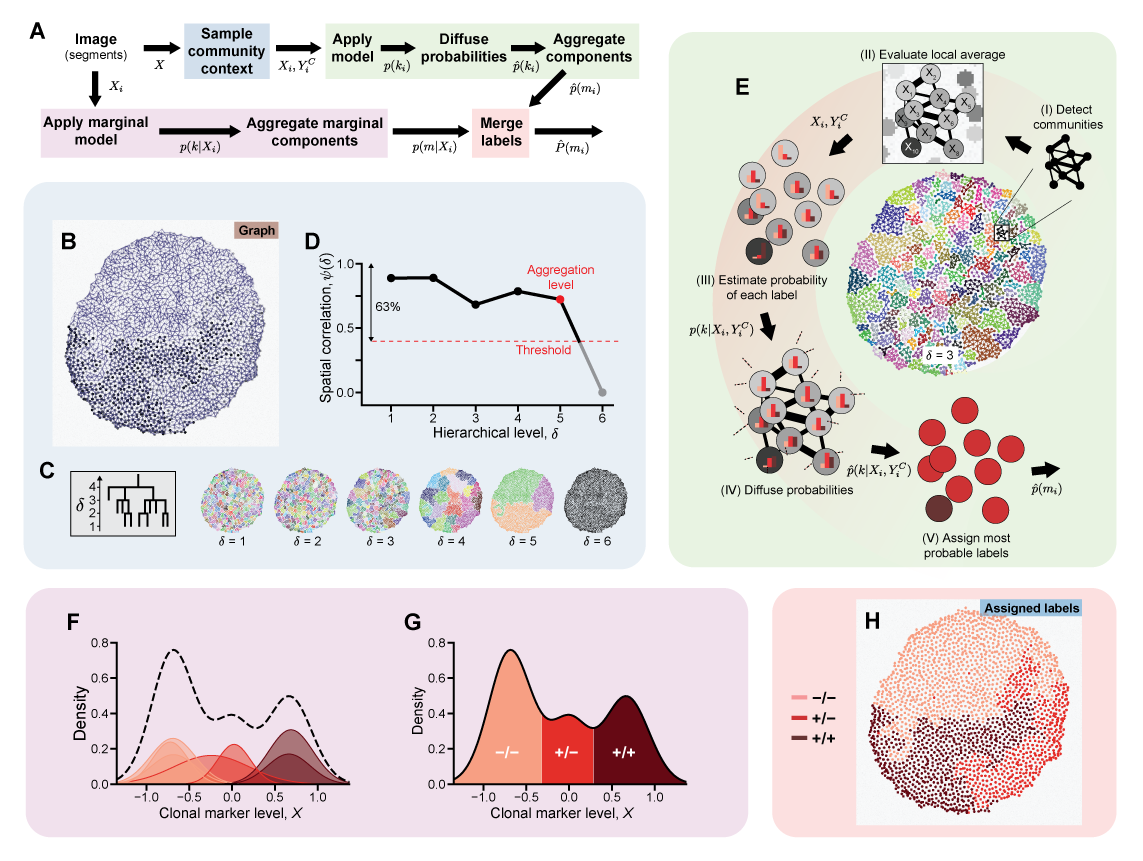
\includegraphics[width=1.0\columnwidth]{./figure_S4}
\caption[Robustness of ribosomopathy simulations to model assumptions.]{\textbf{Reduced protein synthesis capacity diminishes the importance of auxiliary repression over a wide range of model conditions.} Each panel depicts a parameter sweep of the nine-dimensional hyperspace defined by one order of magnitude variation in each of the respective model parameters. For each parameter set, error frequency and percent overexpression were calculated as previously described. They pertain to 50\% reduced repression mimicking auxiliary repressor loss. Error frequency and percent overexpression were calculated independently for conditions of normal and reduced protein synthesis. The difference in error frequency or overexpression between metabolic conditions are shown color-coded, e.g. blue indicates error suppression by reduced protein synthesis. (A-C) Simulations in which the duration of the stimulus input is constant. Shown are the (A) differential error frequencies and (B) differential changes in expression dynamics relative to normal protein synthesis conditions. (C) Differential error frequencies for varying definitions of the success threshold. Each line represents one parameter set, colored by the corresponding range of differential error frequencies. (D) Simulations where a nonzero basal stimulus is applied. (E) Simulations where input duration is increased two-fold by a reduction in protein synthesis capacity. (F) Simulations when an upper bound is placed on the number of sites firing transcription. (G) Simulations when cooperative transcription kinetics are considered.}
\label{fig:metabolism:figS4}
\end{figure}
























% TABLE OF METABOLISM-DEPENDENCE OF TWOSTATE PROPENSITIES
%%%%%%%%%%%%%%%%%%%%%%%%%%%%%%%%%%%%%%%%%%%%%%%%%%%%%%%%%
\begin{table}[h!]
\centering
\small
\caption{Two-state model dependence on environmental conditions}
\label{appendix:supp:metabolism:model:metabolism_twostate}
\begin{tabular}{L{1.75in} C{0.75in} C{1in} C{1.5in}}
\toprule
	& \multicolumn{3}{c}{\bfseries Condition}\\ \cmidrule(lr){2-4}
    \textbf{Reaction} & Normal & Reduced ATP & Reduced ribosomes \\ 
	\midrule  
    Transcription & $k_R$ & $k_R/2$ & $k_R$ \\
    Translation & $k_P$ & $k_P/2$ & $k_P/2$ \\
    Protein decay & $\gamma_P$ & $\gamma_P/2$ & $\gamma_P$  \\ 
    Transcriptional feedback & $\eta_G$ & $\eta_G/4$ & $\eta_G/2$ \\
    Feedback on mRNA & $\eta_R$ & $\eta_R/4$ & $\eta_R/2$ \\
    Feedback on protein & $\eta_P$ & $\eta_P/4$ & $\eta_P/2$  \\
\bottomrule
\end{tabular}
\end{table}







% TABLE OF METABOLISM-DEPENDENCE OF HILL PROPENSITIES
%%%%%%%%%%%%%%%%%%%%%%%%%%%%%%%%%%%%%%%%%%%%%%%%%%%%%
\begin{table}[h!]
\centering
\small
\caption{Hill kinetics model dependence on environmental conditions}
\label{appendix:supp:metabolism:model:metabolism_hill}
%\begin{tabular}{l c c c}
\begin{tabular}{L{1.5in} C{1in} C{1in} C{1.5in}}
\toprule
    & \multicolumn{3}{c}{\bfseries Condition}\\ \cmidrule(lr){2-4}
    \textbf{Reaction} & Normal & Reduced ATP & Reduced ribosomes \\ \cmidrule(lr){1-4}
    Transcription & $k_R$ & $k_R/2$ & $k_R$ \\
    Translation & $k_P$ & $k_P/2$ & $k_P/2$ \\
    Protein decay & $\gamma_P$ & $\gamma_P/2$ & $\gamma_P$  \\
    Feedback on mRNA & $\eta_R$ & $\eta_R/4$ & $\eta_R/2$ \\
    Feedback on protein & $\eta_P$ & $\eta_P/4$ & $\eta_P/2$  \\
\bottomrule
\end{tabular}
\end{table}

The half-maximal occupancy level and Hill coefficients of transcriptional repressors were assumed to be independent of growth rate. Another parameter sweep revealed that despite the incorporation of cooperative binding kinetics, error frequency remains elevated under normal metabolic conditions and is broadly suppressed when metabolism or protein synthesis are reduced (Figs. \ref{fig:metabolism:figS2a}G and \ref{fig:metabolism:figS4}G).